\documentclass{article}

% if you need to pass options to natbib, use, e.g.:
%     \PassOptionsToPackage{numbers, compress}{natbib}
% before loading neurips_2019

% ready for submission
% \usepackage{neurips_2019}

% to compile a preprint version, e.g., for submission to arXiv, add add the
% [preprint] option:
%     \usepackage[preprint]{neurips_2019}

% to compile a camera-ready version, add the [final] option, e.g.:
\usepackage[final]{neurips_2019}
\usepackage{amsmath}

% to avoid loading the natbib package, add option nonatbib:
%     \usepackage[nonatbib]{neurips_2019}

\usepackage[utf8]{inputenc} % allow utf-8 input
\usepackage[T1]{fontenc}    % use 8-bit T1 fonts
\usepackage{hyperref}       % hyperlinks
\usepackage{url}            % simple URL typesetting
\usepackage{booktabs}       % professional-quality tables
\usepackage{amsfonts}       % blackboard math symbols
\usepackage{nicefrac}       % compact symbols for 1/2, etc.
\usepackage{microtype}      % microtypography

\usepackage{amsmath}
\usepackage{tikz}
\usepackage{subcaption} 
\usepackage{pgfplots}
\usepackage{filecontents}

\title{CE7490 Project: Benchmarking Algorithms for Weight Prediction in Weighted Signed Networks}

% The \author macro works with any number of authors. There are two commands
% used to separate the names and addresses of multiple authors: \And and \AND.
%
% Using \And between authors leaves it to LaTeX to determine where to break the
% lines. Using \AND forces a line break at that point. So, if LaTeX puts 3 of 4
% authors names on the first line, and the last on the second line, try using
% \AND instead of \And before the third author name.

\author{%
  Ruihang Wang\\
  % \thanks{Use footnote for providing further information
  %   about author (webpage, alternative address)---\emph{not} for acknowledging
  %   funding agencies.} \\
  School of Computer Science Engineering\\
  Nanyang Technological University\\
  \texttt{ruihang001@e.ntu.edu.sg} \\
  \And
  Meng Shen\\
  % \thanks{Use footnote for providing further information
  %   about author (webpage, alternative address)---\emph{not} for acknowledging
  %   funding agencies.} \\
  School of Computer Science Engineering\\
  Nanyang Technological University\\
  \texttt{meng005@e.ntu.edu.sg} \\
  \And
  Yihang Li\\
  % \thanks{Use footnote for providing further information
  %   about author (webpage, alternative address)---\emph{not} for acknowledging
  %   funding agencies.} \\
  School of Electrical and Electronic Engineering\\
  Nanyang Technological University\\
  \texttt{leah9704@gmail.com} \\
  % examples of more authors
  % \And
  % Coauthor \\
  % Affiliation \\
  % Address \\
  % \texttt{email} \\
  % \AND
  % Coauthor \\
  % Affiliation \\
  % Address \\
  % \texttt{email} \\
  % \And
  % Coauthor \\
  % Affiliation \\
  % Address \\
  % \texttt{email} \\
  % \And
  % Coauthor \\
  % Affiliation \\
  % Address \\
  % \texttt{email} \\
}

\begin{document}

\maketitle

\begin{abstract}
  The abstract paragraph should be indented \nicefrac{1}{2}~inch (3~picas) on
  both the left- and right-hand margins. Use 10~point type, with a vertical
  spacing (leading) of 11~points.  The word \textbf{Abstract} must be centered,
  bold, and in point size 12. Two line spaces precede the abstract. The abstract
  must be limited to one paragraph.
\end{abstract}

\section{Introduction}

[Context] A number of weighted signed networks (WSN) exist in our world while many of them are incomplete. The values for weights prediction are ...

[Existing Solutions] State-of-the-art fairness and goodness. Baselines: Reciprocal, Triadic balance, Triadic Status, Pagerank ....

[Our project]  To better understand theories and master practical skills, we investigate and implement a common set of algorithms and evaluate their performance on real-world datasets. 

The rest of the paper is structured as follows: Section 2 presents related work in this topic. Section 3 describes the overview of our project. Section 4 formulates the problem of weight prediction in weighted signed networks. Section 5 conducted experiments on real-world datasets using different algorithms. Section 6 evaluates the performance of all tested methods. The conclusion is summarized in Section 7.


\section{Related Work}
\textbf{Edge Sign Prediction in SSNs} ...

\textbf{Edge Weight Prediction in Social Networks} ...

\section{Project Overview}

In this project, we extensively investigate and experiment methods for edge weight prediction in weighted signed networks. All algorithms are tested and evaluated on published real-world datasets. Moreover, we try our best to improve the performance on some traditional methods. The finished works are summarized as follows:

\begin{enumerate}
	\item Literature review on OSN and select a topic about predicting weight of edges for weighted signed network.
	
	\item Investigate the state-of-the-art algorithms \emph{fairness-goodness} in [ ] and  studied a common set of baselines for weight prediction.
	
	\item Conducted experiments on each algorithm and reproduce the results mentioned in original paper using real-world dataset.
	
	\emph{Experimental 1 -   Removing one edge prediction} : ...
	
	\emph{Experimental 2 -  Removing N \%-out edge prediction} : ...
	
	\item Evaluate results of different methods.
\end{enumerate}

\section{Problem formulation}

\section{Experiments implementation}


% !TeX root = ../OSN.tex
\subsection{Reciprocal}
As a baseline of weight prediction, reciprocal algorithm takes the 
weight of ($v,u$) as equal to the weight of ($u,v$). When the reciprocal edge 
doesn't exist, the weight of that edge is set to 0. Therefore, the weight of ($u,v$)
is predicted by:

\begin{equation}
W(u,v) =
\begin{cases}
W(v,u),& \text{if $u \rightarrow v$ exist} \\
0,&  \text{otherwise}
\end{cases}
\end{equation}







% !TeX root = ../OSN.tex
\subsection{Triadic balance}
This definition is derived directly from
balance theory according to \cite{}. The algorithm takes the average product of edge weights for all incomplete triads
that the edge ($u,v$) is a part of. Incomplete triads are triads that would form involving
edge ($u,v$) after it is created. To be specific, let $U_n$ and $V_n$ denotes the set of
neighbors of vertex $u$ and $v$, repectively. To find all possible triads, vertexes with
both connections of $u$ and $v$ are obtained by $N = U_n \cap V_n$. When $N = \emptyset$,
the weight of ($u,v$) is set to 0. Then, the weight of ($u,v$)
is predicted by:

\begin{equation}
W(u,v) = 
\begin{cases}
\frac{\sum_{n\in N}W(u,n)+W(n,u)+W(v,n)+W(n,v)}{M}, & \text{if $N \neq \emptyset$} \\
0, & \text{otherwise}
\end{cases}
\end{equation}

where M is number of vertexes in set $N$, $W(u,n), W(n,u), W(v,n), W(n,v)$ are weights of each edge connected
to $u$ or $v$ of vertexes in set $N$, repectively.

% !TeX root = ../OSN.tex

\subsection{Status Theory}

Status theory is derived from \cite{Status}. The prediction made by this measure
is the difference between the status of vertex $u$ and vertex $v$. The status
$\sigma (i)$ of a vertex $i$ is defined as $\sigma (i) = |W^+_{in}(i)| - |W^-_{in}(i)| + |W^-_{out}(i)| - |W^+_{out}(i)|$.
Status increases when receiving positive incoming edges and generating negative 
outgoing edges to other vertices, while decreases when receiving negative edges 
and generating outgoing positive edges. Difference in status measures how much ‘higher’ $u’$s 
status is compared to $v’$s.


% !TeX root = ../OSN.tex

\subsection{Bias and Deserve}
This method is proposed by Mishra and Bhattacharya in \cite{}.
To compute "bias" and "deserve", we should first normalize the ratings (weights),
and keep them in the range of [-1, 1] where 0 is a neutral opinion. Then, we say node $u$ gives a trust-score
of $w_ij$ to node $v$ for a given rating of ($u, v$). The two attributes of a node are 
defined by:

\begin{itemize}
	\item \emph{Bias}: This reflects the expected weight of an outgoing edge.  
	\item \emph{Deserve}: This reflects the expected weight of an incoming edge from an unbiased vertex.
\end{itemize}

Let $d^o(u)$ denotes the set of all outgoing edges from vertex $u$ and likewise,
$d^i(u)$ denotes the set of all incoming links to node $u$. Then, bias (BIAS) and
deserve (DES) are iteratively computed as:

\begin{equation}
    BIAS^{(t+1)}(u)=\frac{1}{å2|d^o(u)|}\sum_{v \in d^o(u)}[W(u,v) - DES^t(v)]
\end{equation}

\begin{equation}
    DES^{(t+1)}(u)=\frac{1}{å2|d^i(u)|}\sum_{v \in d^i(u)}[W(v,u)(1 - X^t(v,u))]
\end{equation}

where $X^t(v,u) = max\{0, BIAS^t(v) \times W(v,u)\}$. The interative formulations
of bias and deserve allow us to predict the weight of (u,v) based on the deserve
value $DES(v)$ of vertex $v$. Thus, the weight is directly predicted by:

\begin{equation}
    W(u,v) = DES(v)
\end{equation}

% !TeX root = ../OSN.tex

\subsection{Page Rank}

We first compute Page Rank ($\omega PR$) value of every vertex(k) in an unsigned graph according to \cite{brin1998anatomy}:

\begin{equation}
\omega PR(k) = \frac{1 - \alpha}{\left | V \right|} + \alpha \sum_{z\in in(k)}\frac{\omega PR(z) * W(z,k)}{\left | out(z) \right |}
\end{equation}

$\alpha$ is the probability called damping factor meaning a person will continue clicking on links(travelling in graph), and we set $\alpha$ to 0.85. $\left |V\right |$ is the number of all nodes. Eventually, $\omega PR(k)$ will converge to the probability that a person will go and stay at node k.

Then we compute edge weight of $(u,v)$ using weighted average of PageRank values:

\begin{equation}
W(u,v) = \frac{\sum_{z\in out(u)} \omega PR(z)*W(u,z) + \sum_{z\in in(v)} \omega PR(z)*W(z,v)}
{\sum_{z\in out(u)}\omega PR(z) + \sum_{z\in in(v)}\omega PR(z)}
\end{equation}



% !TeX root = ../OSN.tex

\subsection{Signed-Hits}

The prediction is computed by using a modified version of HITS for signed network, called Signed-HITS\cite{shahriari2014ranking}. Signed-HITS will compute the hub and authority scores of every node separately on 

% !TeX root = ../OSN.tex

\subsection{Triadic Status}

Imaging there are two nodes named $A$ and $B$, and they are unlinked. What we want to do is to predict the weight of the edge from $A$ to $B$. Suppose that there is another node $X$, and $(A, B, X)$ compose a triangle once $A$ and $B$ are linked. Overall, there are four different triangle-links, as the edge between $X$ and $A$ can go in either direction and similarly for the edge between $X$ and $B$, if the sign of weight is not considered.

\begin{figure}[htbp]
\centering
	\begin{subfigure}{0.2\textwidth}
		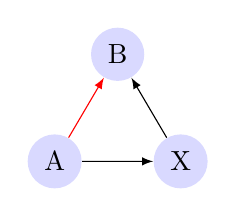
\begin{tikzpicture}
		[scale=0.8,every node/.style={circle,fill=blue!15}]
		  \node (A) at (1,1) {A};
		  \node (B) at (2,2.7)  {B};
		  \node (X) at (3,1)  {X};
		  \draw[->, >=latex, red] (A) edge (B);
		  \draw[->, >=latex] (A) edge (X);
		  \draw[->, >=latex] (X) edge (B);
		\end{tikzpicture}
		\caption{t1}
		\label{t1}
	\end{subfigure}
	\begin{subfigure}{0.2\textwidth}

		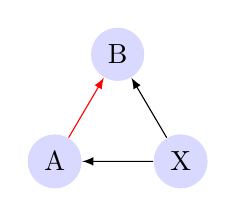
\begin{tikzpicture}
		[scale=0.8,every node/.style={circle,fill=blue!15}]
		\node (A) at (1,1) {A};
		\node (B) at (2,2.7)  {B};
		\node (X) at (3,1)  {X};
		\draw[->, >=latex, red] (A) edge (B);
		\draw[->, >=latex] (X) edge (A);
		\draw[->, >=latex] (X) edge (B);
		\end{tikzpicture}
		\caption{t2}
		\label{t2}
	\end{subfigure}
	\begin{subfigure}{0.2\textwidth}

		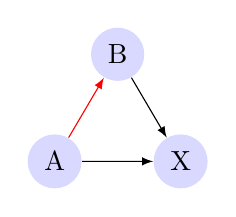
\begin{tikzpicture}
		[scale=0.8,every node/.style={circle,fill=blue!15}]
		\node (A) at (1,1) {A};
		\node (B) at (2,2.7)  {B};
		\node (X) at (3,1)  {X};
		\draw[->, >=latex, red] (A) edge (B);
		\draw[->, >=latex] (A) edge (X);
		\draw[->, >=latex] (B) edge (X);
		\end{tikzpicture}
		\caption{t3}
		\label{t3}
	\end{subfigure}
	\begin{subfigure}{0.2\textwidth}

		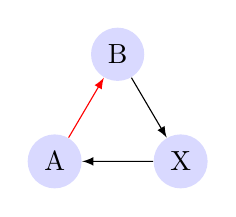
\begin{tikzpicture}
		[scale=0.8,every node/.style={circle,fill=blue!15}]
		  \node (A) at (1,1) {A};
		  \node (B) at (2,2.7)  {B};
		  \node (X) at (3,1)  {X};
		  \draw[->, >=latex, red] (A) edge (B);
		  \draw[->, >=latex] (X) edge (A);
		  \draw[->, >=latex] (B) edge (X);
		\end{tikzpicture}
		\caption{t4}
		\label{t4}
	\end{subfigure}
	\caption{Triadic Status}
	\label{Triadic Status Figure}
\end{figure}

And we predict the weight of the edge $(A, B)$ using three rules:

\begin{enumerate}

\item In Graph t1, the predicted weight of the transitive edge is the sum of the two non-transitive edge weights.

\item In Graph t2 and t3, the predicted weight of a non-transitive edge is the difference of the transitive and the other non-transitive edge weights. 

\item In Graph t4, since it is a cyclic triad, the weight of the missing edge is the negative of the sum of other two edge weights.

\end{enumerate}

In the end, we take the average of predicted weights over all triadic-links that these two nodes are a part of.





% !TeX root = ../OSN.tex

\subsection{Linear Regression}

In this experiment, we use a linear regression model to predict the weight of edge. Our features are generated from some algorithms mentioned above. First, the test edge $e_t$ whose weight is to be predicted is removed from the network. Second, we remove the second edge $e_s$ and predict the weight of $e_s$ from the rest of the edges. And the predicted value of $e_s$ will be the feature and the true value of $e_s$ will be the ground truth. The second step is done multiple times to generate enough samples for training. After training, we use this model to predict the value of the removed edge $e_t$.

% !TeX root = ../OSN.tex

We implemented two series of experiments to evaluate the 
performance of fairness and goodness method on three public 
WSN dataset mentioned above. 

Experiment1:leave-one-out prediction
In these experiments, one weighted edge is removed at a time 
and nine algorithms are implemented to predict the weight of 
test edge, simulating the situation where we want to calculate 
the weight of a non-existed edge. The root-mean-square error 
(RMSE) and Pearson correlation coefficient (PCC) are calculated 
in each loot and the average result is shown in table \ref{table1}. 
Fairness and goodness method achieved almost the best 
performance among all datasets and showed robustness. 
The linear regression result trained by all other features 
is the best one. 

Experiment2:leave-N\%-out prediction
In this part, we removed a larger number of edges to further 
evaluate the performance of F\&G algorithm. We randomly selected 
N\% of the edges, remove them as test edges and predict their 
weight from the rest of network. The value of N range from 10 
to 90 with a step of 10. Figure\ref{figure3}, Figure\ref{figure4} and 
Figure\ref{figure5} showed average RMSE and PCC results in 
the three datasets. F\&G method beats most of the algorithms 
and linear regression method showed robustness and performed 
nearly the best in all datasets. We noticed that performance of
 linear regression method showed stability when the percentage 
 of removed edges varies, meaning that this method can handle 
 networks partly invisible, especilly online networks 
 constrained by privacy items. 


\begin{table}[htbp]
\centering
\caption{Performance of different algorithms for edge weight prediction in leave-one-out experiment on different datasets. Each cell is (RMSE, PCC). Lower RMSE and higher PCC are better.}
	\begin{tabular}{l||c|c|c}
	\toprule
	\textbf{Algorithms}& \textbf{BTCAlphaNet} & \textbf{OTCNet} & \textbf{RFANet}\\ \hline
	& \multicolumn{3}{c}{Existing Algorithms} \\ \hline
	PageRank           & (0.29,0.25) & (0.35,0.30) & (0.21,0.48)\\ \hline
	Bias Deserve      & (0.23,0.60) & (0.28,0.61) & (0.21,0.48)\\ \hline
	Reciprocal         & (0.28,0.44) & (0.33,0.47) & (0.35,0.00)\\ \hline
	Signed HITS       & (0.23,0.66) & (0.27,0.69) & (0.23,0.44)\\ \hline
	Status Theory     & (0.45,0.00) & (0.48,-0.01)& (0.39,-0.15)\\ \hline
	Triadic Balance   & (0.31,0.21) & (0.36,0.28) & (0.24,0.29)\\ \hline
	Triadic Status    & (0.35,0.24) & (0.37,0.42) & (0.32,0.27)\\ \hline
	& \multicolumn{3}{c}{Fairness and Goodness} \\ \hline
	Fairness and Goodness & (0.24,0.60) & (0.28,0.63) & (0.22,0.46)\\ \hline
	& \multicolumn{3}{c}{Linear Regression} \\ \hline
	Linear Regression & (0.22,0.67) & (0.25,0.72) & (0.20,0.54)\\ \hline
	\end{tabular}
	\label{table1}
\end{table}


\begin{filecontents*}{leave_N_rmse_BTCAlphaNet.csv}
percentage,PageRank,Bias_Deserve,Fairness_Goodness,Reciprocal,Signed_HITS,Status_Theory,Triadic_Balance,Triadic_Status,Linear_Regression
10,0.2862059,0.265034144,0.261037457,0.267165064,0.255734648,0.44601129,0.285025372,0.343535,0.26161892
20,0.292917188,0.278317118,0.27363651,0.284231733,0.2676625,0.442839266,0.30377018,0.356856961,0.274874887
30,0.28981181,0.276706453,0.271647122,0.282806161,0.263880247,0.440291816,0.2975907,0.369554382,0.272045979
40,0.29198437,0.275867389,0.27282696,0.296455876,0.265343942,0.431535524,0.304864928,0.39437667,0.271538159
50,0.296086697,0.285137692,0.280603202,0.302069819,0.273881541,0.397503974,0.307107831,0.386513852,0.281900749
60,0.29425471,0.28157068,0.277009576,0.302631283,0.271508214,0.376914071,0.309064461,0.39363739,0.280463814
70,0.299063607,0.292522561,0.2873656,0.311893594,0.279310174,0.378979836,0.315606026,0.396802911,0.288124001
80,0.299979109,0.298713399,0.292424037,0.314659738,0.281180837,0.365892303,0.320763351,0.388727531,0.292594522
90,0.313858609,0.30336673,0.30003005,0.321567433,0.29139145,0.353209865,0.325489449,0.356900946,0.302961136
\end{filecontents*}

\begin{filecontents*}{leave_N_rmse_OTCNet.csv}
percentage,PageRank,Bias_Deserve,Fairness_Goodness,Reciprocal,Signed_HITS,Status_Theory,Triadic_Balance,Triadic_Status,Linear_Regression
10,0.335151341,0.310477855,0.30426336,0.318026367,0.287030277,0.4626312,0.337838956,0.373003723,0.292938484
20,0.347870633,0.325326025,0.316916585,0.333548446,0.301662715,0.47564204,0.346279361,0.38416471,0.305703576
30,0.338595965,0.318813264,0.312393225,0.336789241,0.294172194,0.473299881,0.346940927,0.394102452,0.299969079
40,0.344872106,0.325859136,0.318894397,0.34191172,0.301050849,0.455672839,0.351566938,0.41041154,0.306628896
50,0.339846805,0.324403842,0.318682206,0.346665554,0.301572634,0.437696609,0.348325929,0.41967141,0.308875064
60,0.343532652,0.328489491,0.322570119,0.353472257,0.306942271,0.448583352,0.355882427,0.416653978,0.31238732
70,0.348651608,0.332972538,0.325232271,0.354684021,0.309546946,0.42468728,0.360661617,0.430911557,0.316783801
80,0.34939102,0.338158392,0.332004359,0.359095435,0.314166875,0.40324224,0.363444453,0.43025109,0.321907251
90,0.350782222,0.35526935,0.349576313,0.366474006,0.334772262,0.410662923,0.370006459,0.395412198,0.345462184
\end{filecontents*}

\begin{filecontents*}{leave_N_rmse_RFAnet.csv}
percentage,PageRank,Bias_Deserve,Fairness_Goodness,Reciprocal,Signed_HITS,Status_Theory,Triadic_Balance,Triadic_Status,Linear_Regression
10,0.232410666,0.229617663,0.235285868,0.348678494,0.238945538,0.38114654,0.256234823,0.335533122,0.222348428
20,0.234106197,0.233051523,0.237384184,0.349142862,0.240675521,0.379639524,0.263779467,0.34676506,0.225930518
30,0.23206797,0.229695282,0.234315301,0.347256827,0.238228295,0.375266827,0.26608174,0.352118336,0.222697363
40,0.233809002,0.231834419,0.235958764,0.347765469,0.239322992,0.377100002,0.274133613,0.363017979,0.225006494
50,0.234355193,0.233147123,0.23690299,0.348378403,0.240810398,0.3721229,0.283939319,0.369124995,0.226817743
60,0.236464231,0.236412209,0.239792949,0.348809023,0.24253433,0.372698645,0.295463121,0.379725439,0.229663027
70,0.237053911,0.238929741,0.24109354,0.349037654,0.244069794,0.37170505,0.309303878,0.383238021,0.231771377
80,0.239767649,0.246249791,0.247391051,0.350303916,0.248569772,0.36963466,0.327240562,0.381619836,0.238399125
90,0.249157329,0.262690929,0.261149792,0.349910655,0.259361745,0.362338307,0.342737396,0.364554028,0.25363165
\end{filecontents*}

\begin{filecontents*}{leave_N_pcc_RFAnet.csv}
percentage,PageRank,Bias_Deserve,Fairness_Goodness,Reciprocal,Signed_HITS,Status_Theory,Triadic_Balance,Triadic_Status,Linear_Regression
10,0.45633214,0.47280209,0.45725179,0.03923344,0.43309325,-0.1466368,0.31560244,0.2495895,0.52123316
20,0.4306297,0.44160685,0.42854013,0.03264045,0.40806783,-0.107569,0.26809719,0.215039,0.49298848
30,0.44075809,0.4592817,0.4451822,0.02999544,0.42053632,-0.1293933,0.26711187,0.21256,0.50860711
40,0.431884,0.45104019,0.43789984,0.03600878,0.41809301,-0.0918086,0.24290708,0.18917095,0.49975976
50,0.42893,0.44504304,0.4316053,0.0273973,0.40691194,-0.0977339,0.21032038,0.17657776,0.492099
60,0.4122673,0.42403,0.41133136,0.02469859,0.39634894,-0.0686995,0.17992497,0.14693029,0.47483213
70,0.40577647,0.40996816,0.39823961,0.01834355,0.38256702,-0.0689079,0.14336668,0.12275209,0.46285017
80,0.38857483,0.37500501,0.36519437,0.01433134,0.35973795,-0.0624742,0.10070619,0.08376274,0.43200795
90,0.33569827,0.30244647,0.29502657,0.01114593,0.29365827,-0.0212942,0.0538981,0.04473007,0.36180081
\end{filecontents*}

\begin{filecontents*}{leave_N_pcc_OTCNet.csv}
percentage,PageRank,Bias_Deserve,Fairness_Goodness,Reciprocal,Signed_HITS,Status_Theory,Triadic_Balance,Triadic_Status,Linear_Regression
10,0.323997878,0.458797837,0.468732846,0.430894257,0.55051925,-0.016378973,0.317544935,0.335625259,0.551424884
20,0.314081173,0.43318524,0.453714753,0.403061694,0.528622072,-0.02606627,0.316834788,0.313072951,0.529728897
30,0.360761265,0.465624968,0.476758449,0.377910925,0.559868964,-0.010326893,0.317248716,0.304729722,0.55716076
40,0.329865725,0.4344065,0.445107252,0.344054993,0.529614985,-0.00249936,0.288434743,0.249979705,0.527690337
50,0.349858163,0.437111968,0.443159756,0.302075967,0.524335261,-0.006110895,0.295342312,0.220992299,0.516749531
60,0.341347726,0.423852539,0.431374502,0.262996281,0.507086521,-0.004990537,0.256236968,0.22235416,0.504459184
70,0.320017283,0.40933826,0.417511809,0.2364793,0.489723997,0.013672834,0.225133995,0.131762204,0.491482776
80,0.324214499,0.375372621,0.380373346,0.19443136,0.466547333,0.004259669,0.181288088,0.097108066,0.45929278
90,0.324763464,0.309913302,0.31168425,0.121147265,0.368406218,0.014155932,0.098643912,0.049029838,0.366374839
\end{filecontents*}

\begin{filecontents*}{leave_N_pcc_BTCAlphaNet.csv}
percentage,PageRank,Bias_Deserve,Fairness_Goodness,Reciprocal,Signed_HITS,Status_Theory,Triadic_Balance,Triadic_Status,Linear_Regression
10,0.15991286,0.3919873,0.40415229,0.44566465,0.42241941,-0.0266686,0.25628499,0.2474881,0.43198498
20,0.22123709,0.38052312,0.39507999,0.39575677,0.41851442,0.02557664,0.22459037,0.22074118,0.42061745
30,0.19786691,0.36373454,0.3764956,0.37779074,0.40016534,-0.0071879,0.23532589,0.18670076,0.40692284
40,0.18747658,0.368903,0.37673004,0.33609952,0.40600446,-0.0064677,0.208983,0.15121597,0.41286251
50,0.22043787,0.35714516,0.3669006,0.30521617,0.38639683,-0.0006833,0.21725807,0.16370809,0.38918895
60,0.19238954,0.34658511,0.35658078,0.27109993,0.35781366,-0.019893,0.19161388,0.12309779,0.37063223
70,0.18857408,0.29957216,0.31126149,0.22346306,0.32061861,0.01808413,0.16375077,0.08026381,0.33230114
80,0.17976585,0.28811287,0.29622346,0.18087644,0.31122625,0.00527305,0.1310662,0.06894469,0.32432409
90,0.15581588,0.26082307,0.26241233,0.11491853,0.2495254,-0.0209104,0.08381865,0.05525305,0.27184409
\end{filecontents*}

\begin{figure}[htbp]
	\centering
	\begin{tikzpicture}
	\pgfplotsset{every axis legend/.append style={at={(-0.5,1.6)},anchor=north},every axis y label/.append style={at={(0.03,0.5)}}}
	\begin{axis}[xshift=-2.5cm,title= RMSE BTCAlphaNet ,xlabel=Percentage of removed edges, ylabel=RMSE ,xtick =data,legend columns=5,legend style={font=\footnotesize},font=\footnotesize,width=6cm]
	\addplot table [x=percentage, y=PageRank, col sep=comma] {leave_N_rmse_BTCAlphaNet.csv};
	\addplot table [x=percentage, y=Bias_Deserve, col sep=comma] {leave_N_rmse_BTCAlphaNet.csv};
	\addplot table [x=percentage, y=Fairness_Goodness, col sep=comma] {leave_N_rmse_BTCAlphaNet.csv};
	\addplot table [x=percentage, y=Reciprocal, col sep=comma] {leave_N_rmse_BTCAlphaNet.csv};
	\addplot table [x=percentage, y=Signed_HITS, col sep=comma] {leave_N_rmse_BTCAlphaNet.csv};
	\addplot table [x=percentage, y=Status_Theory, col sep=comma] {leave_N_rmse_BTCAlphaNet.csv};
	\addplot table [x=percentage, y=Triadic_Balance, col sep=comma] {leave_N_rmse_BTCAlphaNet.csv};
	\addplot table [x=percentage, y=Triadic_Status, col sep=comma] {leave_N_rmse_BTCAlphaNet.csv};
	\addplot table [x=percentage, y=Linear_Regression, col sep=comma] {leave_N_rmse_BTCAlphaNet.csv};
	\end{axis}
	\begin{axis}[xshift=5cm,title= PCC BTCAlphaNet ,xlabel=Percentage of removed edges, ylabel=PCC ,xtick =data,legend columns=5,legend style={font=\footnotesize},font=\footnotesize,width=6cm]
	\addplot table [x=percentage, y=PageRank, col sep=comma] {leave_N_pcc_BTCAlphaNet.csv};
	\addplot table [x=percentage, y=Bias_Deserve, col sep=comma] {leave_N_pcc_BTCAlphaNet.csv};
	\addplot table [x=percentage, y=Fairness_Goodness, col sep=comma] {leave_N_pcc_BTCAlphaNet.csv};
	\addplot table [x=percentage, y=Reciprocal, col sep=comma] {leave_N_pcc_BTCAlphaNet.csv};
	\addplot table [x=percentage, y=Signed_HITS, col sep=comma] {leave_N_pcc_BTCAlphaNet.csv};
	\addplot table [x=percentage, y=Status_Theory, col sep=comma] {leave_N_pcc_BTCAlphaNet.csv};
	\addplot table [x=percentage, y=Triadic_Balance, col sep=comma] {leave_N_pcc_BTCAlphaNet.csv};
	\addplot table [x=percentage, y=Triadic_Status, col sep=comma] {leave_N_pcc_BTCAlphaNet.csv};
	\addplot table [x=percentage, y=Linear_Regression, col sep=comma] {leave_N_pcc_BTCAlphaNet.csv};

	\end{axis}
	\end{tikzpicture}
	\caption{BTCAlphaNet}
	\label{figure3}
\end{figure}
\begin{figure}[htbp]
	\centering
	\begin{tikzpicture}
	\pgfplotsset{every axis legend/.append style={at={(-0.5,1.6)},anchor=north},every axis y label/.append style={at={(0.03,0.5)}}}
	\begin{axis}[xshift=-2.5cm,title= RMSE OTCNet ,xlabel=Percentage of removed edges, ylabel=RMSE ,xtick =data,legend columns=5,legend style={font=\footnotesize},font=\footnotesize,width=6cm]
	\addplot table [x=percentage, y=PageRank, col sep=comma] {leave_N_rmse_OTCNet.csv};
	\addplot table [x=percentage, y=Bias_Deserve, col sep=comma] {leave_N_rmse_OTCNet.csv};
	\addplot table [x=percentage, y=Fairness_Goodness, col sep=comma] {leave_N_rmse_OTCNet.csv};
	\addplot table [x=percentage, y=Reciprocal, col sep=comma] {leave_N_rmse_OTCNet.csv};
	\addplot table [x=percentage, y=Signed_HITS, col sep=comma] {leave_N_rmse_OTCNet.csv};
	\addplot table [x=percentage, y=Status_Theory, col sep=comma] {leave_N_rmse_OTCNet.csv};
	\addplot table [x=percentage, y=Triadic_Balance, col sep=comma] {leave_N_rmse_OTCNet.csv};
	\addplot table [x=percentage, y=Triadic_Status, col sep=comma] {leave_N_rmse_OTCNet.csv};
	\addplot table [x=percentage, y=Linear_Regression, col sep=comma] {leave_N_rmse_OTCNet.csv};
	\end{axis}
	\begin{axis}[xshift=5cm,title= PCC OTCNet ,xlabel=Percentage of removed edges, ylabel=PCC ,xtick =data,legend columns=5,legend style={font=\footnotesize},font=\footnotesize,width=6cm]
	\addplot table [x=percentage, y=PageRank, col sep=comma] {leave_N_pcc_OTCNet.csv};
	\addplot table [x=percentage, y=Bias_Deserve, col sep=comma] {leave_N_pcc_OTCNet.csv};
	\addplot table [x=percentage, y=Fairness_Goodness, col sep=comma] {leave_N_pcc_OTCNet.csv};
	\addplot table [x=percentage, y=Reciprocal, col sep=comma] {leave_N_pcc_OTCNet.csv};
	\addplot table [x=percentage, y=Signed_HITS, col sep=comma] {leave_N_pcc_OTCNet.csv};
	\addplot table [x=percentage, y=Status_Theory, col sep=comma] {leave_N_pcc_OTCNet.csv};
	\addplot table [x=percentage, y=Triadic_Balance, col sep=comma] {leave_N_pcc_OTCNet.csv};
	\addplot table [x=percentage, y=Triadic_Status, col sep=comma] {leave_N_pcc_OTCNet.csv};
	\addplot table [x=percentage, y=Linear_Regression, col sep=comma] {leave_N_pcc_OTCNet.csv};

	\end{axis}
	\end{tikzpicture}
	\caption{OTCNet}
	\label{figure4}
\end{figure}
\begin{figure}[htbp]
	\centering
	\begin{tikzpicture}
	\pgfplotsset{every axis legend/.append style={at={(-0.5,-0.8)},anchor=south},every axis y label/.append style={at={(0.03,0.5)}}}
	\begin{axis}[xshift=-4cm,title= RMSE RFAnet ,xlabel=Percentage of removed edges, ylabel=RMSE ,xtick =data,legend columns=5,legend style={font=\footnotesize},font=\footnotesize,width=6cm]
	\addplot table [x=percentage, y=PageRank, col sep=comma] {leave_N_rmse_RFAnet.csv};
	\addplot table [x=percentage, y=Bias_Deserve, col sep=comma] {leave_N_rmse_RFAnet.csv};
	\addplot table [x=percentage, y=Fairness_Goodness, col sep=comma] {leave_N_rmse_RFAnet.csv};
	\addplot table [x=percentage, y=Reciprocal, col sep=comma] {leave_N_rmse_RFAnet.csv};
	\addplot table [x=percentage, y=Signed_HITS, col sep=comma] {leave_N_rmse_RFAnet.csv};
	\addplot table [x=percentage, y=Status_Theory, col sep=comma] {leave_N_rmse_RFAnet.csv};
	\addplot table [x=percentage, y=Triadic_Balance, col sep=comma] {leave_N_rmse_RFAnet.csv};
	\addplot table [x=percentage, y=Triadic_Status, col sep=comma] {leave_N_rmse_RFAnet.csv};
	\addplot table [x=percentage, y=Linear_Regression, col sep=comma] {leave_N_rmse_RFAnet.csv};
	\end{axis}
	\begin{axis}[xshift=4cm,title= PCC RFAnet ,xlabel=Percentage of removed edges, ylabel=PCC ,xtick =data,legend columns=5,legend style={font=\footnotesize},font=\footnotesize,width=6cm]
	\addplot table [x=percentage, y=PageRank, col sep=comma] {leave_N_pcc_RFAnet.csv};
	\addplot table [x=percentage, y=Bias_Deserve, col sep=comma] {leave_N_pcc_RFAnet.csv};
	\addplot table [x=percentage, y=Fairness_Goodness, col sep=comma] {leave_N_pcc_RFAnet.csv};
	\addplot table [x=percentage, y=Reciprocal, col sep=comma] {leave_N_pcc_RFAnet.csv};
	\addplot table [x=percentage, y=Signed_HITS, col sep=comma] {leave_N_pcc_RFAnet.csv};
	\addplot table [x=percentage, y=Status_Theory, col sep=comma] {leave_N_pcc_RFAnet.csv};
	\addplot table [x=percentage, y=Triadic_Balance, col sep=comma] {leave_N_pcc_RFAnet.csv};
	\addplot table [x=percentage, y=Triadic_Status, col sep=comma] {leave_N_pcc_RFAnet.csv};
	\addplot table [x=percentage, y=Linear_Regression, col sep=comma] {leave_N_pcc_RFAnet.csv};

	\legend{$$Page Rank, $$Bias Deserve, $$Fairness Goodness, $$Reciprocal, $$Signed HITS, $$Status Theory, $$Triadic Balance, $$Triadic Status, $$Linear Regression}
	\end{axis}
	\end{tikzpicture}
	\caption{RFAnet}
	\label{figure5}
\end{figure}









\section{Conclusion}


\bibliographystyle{unsrt}
\bibliography{bib/ref}



\end{document}